\begin{enumerate}[label=\thesubsection.\arabic*,ref=\thesubsection.\theenumi]
   % 
    \item Let $ABCD$ be a unit square. Suppose $M$ and $N$ are points on $BC$ and $CD$, respectively, such that the perimeter of triangle $MCN$ is $2$. Let $O$ be the circumcenter of triangle $MAN$, and $P$ be the circumcenter of triangle $MON$. If $\left(\frac{OP}{OA}\right)^2 = \frac{m}{n}$ for some relatively prime positive integers $m$ and $n$, find the value of $m + n$.\hfill(IOQM 2015)
    
    \item In triangle  $ABC$, point $ A_1 $ lies on side $ BC $ and point $B_1$ lies on side $ AC $. Let  $P$ and $ Q $ be points on segments 
$AA_1$ and $BB_1 $, respectively, such that   $PQ \parallel AB$.
Let
 $P_1$ be a point on line  $PB_1$ such that $B_1$ lies strictly between 
$P$ and $P_1$, and $\angle PP_1C$ = $\angle BAC$. Similarly, let $Q_1$ 
be a point on line $QA_1$ such that $A_1$ lies strictly between $Q$ and 
$Q_1$, and $ \angle CQ_1Q$ = $\angle CBA $.
Prove that points $P, Q, P_1,$ and $Q_1$ are concyclic.
\hfill(IMO 2019)


\item Let $D$ be an interior point of the acute triangle $ABC$ with $AB > AC$ so that $\angle DAB = \angle CAD$. The point $E$ on the segment $AC$ satisfies $\angle ADE=\angle BCD$, the point $F$ on the segment $AB$ satisfies $\angle FDA=\angle DBC$, and the point $X$ on the line $AC$ satisfies $CX=BX$. let $O_{1}$ and $O_{2}$ be the circumcentres of the triangles $ADC$ and $EXD$, respectively. Prove that the lines $BC,EF$ and $O_{1} O_{2}$ are concurrent.
 \hfill(IMO 2021)

\item $ABCD$ is cyclic. The feet of the perpendicular from $D$ to the lines $AB$, $BC$, $CA$ are $P, Q,R $ respectivel$y$. Show that the angle bisectors of $ ABC$ and $CDA$ meet on the line $AC$ iff $RP = RQ$.\hfill(IMO 2003)
%
\item In the convex quadrilateral $ABCD$, the diagonals $AC$ and $BD$ are perpendicular and the opposite sides $AB$ and $DC$ are not parallel. Suppose that the point $P$, where the perpendicular bisectors of $AB$and $DC$ meet, is inside $ABCD$. Prove that $ABCD$ is a cyclic quadrilateral if and only if the triangles $ABP$ and $CDP$ have equal areas.

	\hfill(IMO  1998) 
\item Consider five points $A,B,C,D$ and $E$ such that $ABCD$ is a parallelogram and $BCED$ is a cyclic quadrilateral. Let $l$ be a line passing through $A$. Suppose that $l$ intersts the interior of the segment $DC$ at $F$ and intersects line $BC$ at $G$. Suppose also that $EF=EG=EC$. Prove that $l$ is the bisector of angle $DAB$.\hfill(IMO  2007)
		
\item Let $P$ be a point inside triangle $ABC$ such     that                                         
\begin{align*}                                      
	\angle{APB}-\angle{ACB}=\angle{APC}-\angle{ BC}.
 \end{align*}                                       
Let $D$, $E$ be the incenters of triangles $APB$, $APC$, respectively. Show that $AP$, $BD$, $CE$ meet at a point.\hfill(IMO  1996)
\item Let $ABCDEF$ be a convex hexagon such that $A$ is parallel to $DE$, $BC$ is parallel to $EF$, and $CD$ is parallel to $FA$. Let $R_A$, $R_C$, $R_E$ denote the circumradii of triangles $FAB$, $BCD$, $DEF$, respectively, and let $P$ denote the perimeter of the hexagon. Prove that            \hfill(IMO  1996)
\begin{align*}                                            R_A+R_C+R_E\geq\frac{p}{2}.  
\end{align*}
\item The angle at $A$ is the smallest angle of triangle $ABC$. The point $B$ and $C$ divide the circumcircle of the triangle into two arcs. Let $U$ be an interior point of the arc between $B$ and $C$ which does not contain $A$. The perpendicular bisectors of  $AB$ and $AC$ meet the line $AU$ at $V$ and $W$, respctively. The lines $BV$ and $CW$ meet at $T$. Show that
\hfill(IMO  1997)
 \begin{align*}
AU=TB+TC.
 \end{align*}                                   
\item Let $P=A_1A_2 \dots A_k$ be a convex polygon in the plane. The vertices $A_1, A_2,\dots A_k $ have integral coordinates and lie on a circle. Let $S$ be the area of $P$. An odd positive integer $n$ is given such that the squares of the side lengths of $P$ are integers divisible by $n$. Prove that $2S$ is an integer divisible by $n$.\hfill(IMO  2016)
\item Let $I$ be the circumcircle of acute-angled triangle $ABC$. Points $D$ and $E$     lie on segments $AB$ and $AC$ respectively, such that $AD=AE$. The perpendicular bisectors of $BD$ and $CE$ intersect the minor arcs $AB$ and $AC$ of $I$ at points $F$ and $G$ respectively. Prove that the lines $DE$ and $FG$ are parallel (or are the same line).\hfill (IMO  2018)
\item In the plane let $C$ be a circle, $L$ a line  tangent to the circle $C$, and $M$ a point on $L$. Find the locus of all points $P$ with the following property: there exists two points $Q,R$ on $L$ such that $M$ is the midpoint of $QR$ and $C$ is the inscribed circle of triangle $PQR$.  \hfill(IMO  1992)
\item Let $D$ be a point inside acute triangle $ABC$ such that $\angle ADB$ $=$ $\angle ACB$ $+$ $\pi/2$ and $AC \cdot BD = AD \cdot BC$.
 
\begin{enumerate}
\item Calculate the ratio $(AB \cdot CD) / (AC \cdot B)$.
\item Prove that the tangents at $C$ to the circumcircles of $\triangle ACD$ and $\triangle BCD$ are perpendicular. \hfill(IMO  1993)
\end{enumerate}
\item In a triangle $ABC$, let $I$ denote the incenter. Let the lines $AI$, $BI$, and $CI$ intersect the incircle at $P$, $Q$, and $R$, respectively. If $\angle BAC = 40\degree$, what is the value of $\angle QPR$ in degrees?\hfill(PRMO 2014)
\item $AB$ is tangent to the circles $CAMN$ and $NMBD$. $M$ lies between $C$ and $D$ on the line $CD$, and $CD$ is parallel to $AB$. The chords $NA$ and $CM$ meet at $P$; the chords $NB$ and $MD$ meet at $Q$. The rays $CA$ and $DB$ meet at $E$. Prove that $PE = QE$.

	\hfill(IMO 2000)
\item $O$ and $I$ are the circumcentre and incentre of $\triangle ABC$ respectively. Suppose $O$ lies in the interior of $\triangle ABC$ and $I$ lies on the circle passing through $B$, $O$, and $C$. What is the magnitude of $\angle BAC$ in degrees?\hfill(PRMO 2012)
    \item In rectangle $ ABCD $, $ AB = 8 $ and $ BC = 20 $. Let $ P $ be a point on $ AD $ such that $ \angle BPC = 90\degree $. If $ r_1, r_2, r_3 $ are the radii of the incircles of triangles $ APB, BPC $, and $ CPD $, what is the value of $ r_1 + r_2 + r_3 $? \hfill(PRMO 2015)
\item The circle $ \omega $ touches the circle $ \Omega $ internally at $ P $. The center $ O $ of $ \Omega $ is outside $ \omega $. Let $XY$ be a diameter of $ \Omega $ which is also tangent to $ \omega $. Assume $ PY > PX $. Let $ PY $ intersect $ \omega $ at $ Z $. If $ YZ = 2PZ $, what is the magnitude of $ \angle LPYX $ in degrees? 

	\hfill(PRMO 2015)
\item
 Let $I$ be the incentre of acute triangle $ABC$ with $AB$ $\neq AC$. 
The incircle $\omega$ of $ABC$ is tangent to sides $ BC$, $CA$, and $AB$
 at points $D$,  $E$, and $F$, respectively. 
The line 
through $D$ perpendicular to $EF$ meets $\omega$ again at $R$. Line $AR$
 meets $\omega$ again at $P$. The circumcircles of triangles $PCE$ and 
$PBF$ meet again at $Q$.
Prove that lines $DI$ and $PQ$ meet on the line through $ A$ that is perpendicular to $AI$.
\hfill(IMO 2019)
\item Let $r$ be a circle with centre $I$, and $ABCD$ a convex quadrilateral such that each of the segments $AB,BC,CD$ and $DA$ is a tangent to $r$. Let $\Omega$ be the circumcircle of the triangle $AIC$. The extension of $BA$ beyond $A$ meets $\Omega$ at $X$, and the extension of $BC$ beyond $C$ meets $\Omega$ at $Z$. The extensions of $AD$ and $CD$ beyond $D$ meet $\Omega$ at $Y$ and $T$, respectively. Prove that
\begin{align*}
    AD+DT+TX+XA=CD+DY+YZ+ZC
\end{align*}
 \hfill(IMO 2021)
 \item
Let $ABCDE$  be a convex pentagon such that  $BC = DE$.  Assume that there is a point  $T$  inside  $ABCDE$ with  $TB = TD$,  $TC = TE$  and  $\angle{ABT} = \angle{TEA}$.  Let line  $AB$  intersect 
lines $CD$  and  $CT$  at points  $P$  and $Q$,  respectively. Assume that the points  $P, B, A, Q$  occur on their line in that order. Let line  $AE$  intersect lines  $CD$  and  $DT$  at points  $R$  and  $S$,  respectively. Assume 
that the points $ R, E, A, S $ occur on their line in that order. Prove that the points $ P, S, Q, R $ lie on a circle. \hfill(IM0 2022)
\item
Let  $ABC$ be an acute-angled triangle with  $AB \leq AC$. Let $\Omega$  be the circumcircle of  $ABC$.  Let  $S$ be the midpoint of the arc  $CB$  of  $\Omega$ containing $A$.  The perpendicular from $A$  to  $BC$ meets  $BS$  at  $D$  and meets  $\Omega$  again at$ E \neq A$. The line through $
D$ parallel to  $BC$  meets line  $BE$ at  $L$.  Denote the circumcircle of triangle  $BDL$  by  $\omega$.  Let  $\omega$  meet  $\Omega$  again at  $P \neq B$. Prove that the line tangent to $\omega$ at  $P$  meets line $BS$  on the internal angle bisector of  $\angle{BAC}$. \hfill(IMO 2023)
\item
Let  $ABC$  be an equilateral triangle. Let $A_{1}, B_{1}, C_{1}$  be interior points of  $ABC$  such that $ BA_{1} = A_{1}C, CB_{1} = B_{1}A, AC_{1} = C_{1}B,$  and $\angle{BAC} + \angle{CB_{1}A} + \angle{AC_{1}B} = 480^{\circ}.$  Let $ BC_{1}$ and $CB_{1}$  meet at $A_{2}$,  let  $CA_{1}$ and  $A
C_{1}$  meet at  $B_{2}$,  and let  $AB_{1}$ and  $BA_{1}$  meet at  $C_{2}$. Prove that if triangle  $A_{1}B_{1}C_{1}$  is scalene, then the three circumcircles of triangles $AA_{1}A_{2}, BB_{1}B_{2}$  and  $CC_{1}C_{2}$ all pass through two common points.
$\brak{\text{Note: no 2 sides have equal length.}}$ \hfill(IMO 2023)
\item
Let  $ABC$  be a triangle with $ AB \leq AC \leq BC $.  Let the incentre and incircle of triangle   $ABC$  be  $I$ and  $\omega$, respectively. Let $X$ be the point on line  $BC$  different from  $C$  such that the line   through  $X$  parallel to  $AC$  is tangent to  $\omega$.  Similarly, let  $
Y$ be the point on line  $BC$  different from  $B$  such that the line through  $Y$ parallel to  $AB$  is tangent to  $\omega$.  Let $AI$  intersect the circumcircle of  triangle $ABC$  again at  $P \neq A$. Let  $K$  and $L$  be the midpoints of  $AC$  and  $AB$,  respectively.  Prove that  $\angle{KIL} + \angle{YPX} = 180^{\circ}.$ 

\hfill(IMO 2024)
\item In a triangle $ ABC $, let $ H $, $ I $, and $ O $ be the orthocenter, incenter, and circumcenter, respectively. If the points $ B $, $ H $, $ I $, and $ C $ lie on a circle, what is the magnitude of $ \angle BOC $ in degrees?\hfill(PRMO 2013)
\item Let $ S $ be a circle with center $ O $. A chord $ AB $, not a diameter, divides $ S $ into two regions $ R_1 $ and $ R_2 $. Let $ S_1 $ be a circle with center in $ R_1 $ touching $ AB $, the circle $ S $ internally. Let $ S_2 $ be a circle with center in $ R_2 $ touching $ AB $ at $ Y $, the circle $ S $ internally, and passing through the center of $ S $. The point $ X $ lies on the diameter passing through the center of $ S_2 $, and $ \angle YXO = 30\degree $. If the radius of $ S_2 $ is 100, then what is the radius of $ S $?\hfill(PRMO 2013)
\item $BC$ is a diameter of a circle with center $O$. $A$ is any point on the circle with $\angle AOC > 60\degree$. $EF$ is the chord which is the perpendicular bisector of $AO$. $D$ is the midpoint of the minor arc $AB$. The line through $O$ parallel to $AD$ meets $AC$ at $J$. Show that $J$ is the incenter of triangle $CEF$.\hfill(IMO 2002)
\item Let $ABCD$ be a convex quadrilateral such that the line $CD$ is a  tangent to the circle on $AB$ as diameter. Prove that the line $AB$ is a tangent to the  circle on $CD$ as diameter if and only if the lines $BC$ and $AD$ are parallel.\hfill(IMO 1984)
\item let $A$ be one of the two distinct points of intersection of two unequal coplanar tangents to the circles $C_1$ and $C_2$ with centers $ O_1$ and $O_2$, respectively. One of the common tangents to the circles touches $C_1$ at $P_1$ and $C_2$ at $P_2$, while the other touches $C_1$ at $Q_1$ and $C_2$ at $Q_2$.  Let $M_1$ be the midpoint of $P_1Q_1$, $M_2$ be the midpoint of $P_2Q_2$. Prove that $\angle O_1AO_2 =\angle M_1AM_2$.\hfill(IMO 1983)
     \item $A$ circle has center on the side $AB$ of the cyclic quadrilateral $ABCD$. The other three sides are tangent to the circle. Prove that $AD+BC = AB$.\hfill(IMO 1985)
\item A circle with center $O$ passes through the vertices $A$ and $C$ of triangle $ABC$ and intersects the segments $AB$ and $BC$ again at distinct points $K$ and $N$ respectively. The circumscribed circle of the triangle $ABC$ and $EBN$ intersect at exactly two distinct points $B$ and $M$. Prove that angle $OMB$ is a right angle.\hfill(IMO 1985)
\item Three congruent circles have a common point $O$ and lie inside     a given triangle. Each circle touches a pair of sides of the triangle. Prove that the incenter and the circumcenter of the triangle and   the point $O$  are collinear. \hfill(IMO  1981)     
\item A non-isosceles triangle $A_1 A_2 A_3$ is given with sides $a_1,a_2,a_3$ ($a_i$ is the side opposite $A_i$). For all $i = 1, 2, 3, M_i$ is the midpoint of side $a_i$ and $T_i$ is the point where     the incircle touches side $a_i$. Denote by $S_i$ the reflection of $T_i$ in the interior bisector of angle $A_i$. Prove that the lines $M_1S_1$, $ M_2S_2$ and $M_3S_3$ are concurrent.\hfill(IMO  1982)
    \item In an acute-angled triangle $ABC$ the interior bisector of the angle $A$ intersects $BC$ at $L$ and intersects the circumcircle of $ABC$ again at $N$. From point $L$ perpendiculars are drawn to $AB$ and $AC$, the feet of these perpendiculars being $K$ and $M$ respectively. Prove that the quadrilateral $AKNM$ and the triangle $ABC$ have equal areas.

	    \hfill(IMO  1987)
    \item Consider two coplanar circles of radii $R$ and $r$ $\brak{R > r}$ with the same center. Let $P$ be a fixed point on the smaller circle and $B$ a variable point on the larger circle. The line $BP$ meets the larger circle again at $C$. The perpendicular $l$ to $BP $ at $P$ meets the smaller circle again at $A$. (If $l$ is tangent to the circle at $P$ then $A = P$).
\hfill(IMO  1988)
\begin{enumerate}
	\item  Find the set of values of $BC^2+CA^2+AB^2$ 
	\item  Find the locus of the midpoint of $BC$.
\end{enumerate}
\item  Let the excircle of triangle $ABC$ opposite the vertex $A$ be tangent to the side $BC$ at the point $A_1$. Define the points $B_1$ on $CA$ and $C_1$ on $AB$ analogously, using the excircles opposite $B$ and $C$ respectively. Suppose that the circumcentre of triangle $A_1B_1C_1$, lies on the circumcircle of triangle $ABC$. Prove that triangle $ABC$ is right-angled. 
	(The excircle of triangle $ABC$ opposite the vertex $A$ is the circle that is tangent to the line segment $BC$, to the ray $AB$ beyond $B$, and to the ray $AC$ beyond $C$. The excircles opposite $B$ and $C$ are similarly defined. \hfill(IMO  2013)
\item  Convex quadrilateral $ABCD$ has $\angle ABC= \angle CDA = 90 \degree$. Point $H$ is the foot of the perpendicular from $A$ to $BD$. Points $S$ and $T$ lie on sides $AB$ and $AD$ respectively, such that $H$ lies inside triangle $SCT$ and $\angle CHS- \angle CSB = 90 \degree, \angle THC- \angle DTC = 90\degree$.
	Prove that line $BD$ is tangent to the circumcircle of triangle $TSH$.
	\hfill(IMO  2014)
\item   Points $P$ and $Q$ lie on side $BC$ of acute-angled triangle $ABC$ so that $\angle PAB= \angle BCA$ and $\angle CAQ=\angle ABC.$ Points $M$ and $N$ lie on lines $AP$ and $AQ,$ respectively, such that $P$ is the midpoint of $AM,$ and $Q$ is the midpoint of $AN.$ Prove that lines $BM$ and $CN$ intersect on circumcircle of triangle $ABC$ \hfill(IMO  2014)
\item   Let $ABC$ be an acute triangle with $AB > AC$. Let $I$ be its circumcircle, $H$ its orthocentre, and $F$ the foot of the altitude from $A$. Let $M$ be the midpoint of $BC$. Let $Q$ be the point on $T$ such that $\angle HQA= 90$, and let $K$ be the point on $T$ such that $\angle HKQ=90\degree.$ Assume that the points $ A, B, C, K$ and $Q$ are all different, and lie on $T$ in this order.
	Prove that the circumcircles of triangles $KQH$ and $FKM$ are tangent to each other. \hfill(IMO 2015)
\item  Triangle $ABC$ has circumcircle $\Omega$ and circumcentre $O$. A circle $T$ with centre $A$ intersects the segment $BC$ at points $D$ and $E$, such that $B, D, E $ and $C$ are all different and lie on line $BC$ in this order. Let $F$ and $G$ be the points of intersection of $T$ and $\Omega$ such that $A, F, B, C$ and $G$ lie on $\Omega$ in this order. Let $K $ be the second point of intersection of the circumcircle of triangle $BDF$ and the segment $AB$. Let $L$ be the second point of intersection of the circumcircle of triangle $CGE$ and the segment $CA$.
	Suppose that the lines $FK$ and $GL$ are different and intersect at the point $X$. Prove that $X$ lies on the line $AO$. \hfill(IMO  2015)
\item In an acute-angled triangle $ABC$, the internal bisector of angle $A$ meets the circumcircle of the triangle again at $A_1$. Points $B_1$ and $C_1$ are defined similarly. Let $A_0$ be the point of intersection of the line $AA_1$ with the external bisectors of angles $B$ and $C$. Points $B_0$ and $C_0$ are defined similarly. Prove that
\begin{enumerate}
\item The area of the triangle $A_0$ $B_0C_0$ is twice the area of the hexagon $AC_1BA_1CB_1$
\item  The area of the triangle $A_0B_0C_0$ is at least four times the area of the triangle $ABC$. 

	\hfill(IMO  1989)
\end{enumerate}
   \item Chords $AB$ and $CD$ of a circle intersect at a point $E$ inside the circle. Let $M$ be an interior point of the segment $EB$. The tangent line at $E$ to the circle through $D, E$ and $M$ intersects the lines $BC$ and $AC$ at $F$ and $G$ respectively. If $\frac{AM}{AB}=t$,
  find $ \frac{EG}{EF}$  
	  in terms of $t$.\hfill(IMO  1990)
\item In triangle $ABC$, $AB = AC$. A circle is tangent internally to the circumcircle of triangle $ABC$ and also to sides $AB, AC$ at $P, Q$, respectively. Prove that the midpoint of segment $PQ$ is the center of the incircle of triangle $ABC.$\hfill(IMO  1978)
\item Two circles in a plane intersect. Let $A$ be one of the points of intersection. Starting simultaneously from $A$ two points move with constant speeds, each point travelling along its own circle in the same sense. The two points return to $A$ simultaneously after one revolution. Prove that there is a fixed point $P$ in the plane such that, at any time, the distances from $P$ to the moving points are equal.\hfill(IMO  1979) 
\item Let $I$ be the incenter of triangle $ABC$. Let the incircle of $ABC$ touch the sides $BC$,$CA$, and $AB$ at $K$, $L$, and $M$, respectively. The line through $B$ parallel to $MK$ meets the lines $LM$ and $LK$ at $R$ and $S$ respectively. Prove that angle $RIS$ is acute.\hfill(IMO  1998)
%
\item Two circles ${G_{1}}$ and ${G_{2}}$ are contained inside the circle $G$, and are tangent to $G$ at the distinct points $M$ and $N$, respectively. ${G_{1}}$ passes through the center of ${G_{2}}$. The line passing through the two points of intersection of ${G_{1}}$ and ${G_{2}}$ meets $G$ at $A$ and $B$. The lines $MA$ and $MB$ meet ${G_{1}}$ at $C$ and $D$ respectively. Prove that $CD$ is tangent to ${G_{2}}$.\hfill(IMO  1999)
                      	
\item ${A_{1}} {A_{2}} {A_{3}}$ is an acute-angled triangle. The foot of the altitude from ${A_{i}}$ is ${K_{i}}$ and the incircle touches the side opposite ${A_{i}}$ at ${L_{i}}$. The line ${K_{1}}{K_{2}}$ is reflected in the line ${L_{1}}{L_{2}}$. Similarly, the line ${K_{2}}{K_{3}}$ is reflected in ${L_{2}}{L_{3}}$ and ${K_{3}}{K_{1}}$ is reflected in ${L_{3}}{L_{1}}$. Show that the three new lines form a triangle with vertices on the incircle.\hfill(IMO  2000)
\item Let $ABC$ be an acute-angled triangle  with $AB$ $\neq$ $AC$. The circle with diameter $BC$ intersects the sides $AB$ and $AC$ at $M$ and $N$ respectively. Denote by $O$ the midpoint of the side $BC$. The bisectors of the angles $BAC$ and $MON$ intersect at $R$. Prove that the circumcircles of the triangles $BMR$ and $CNR$ have a common point on the side $BC$. \hfill(IMO  2004)
 \item In a convex quadrilateral $ABCD$ the diagonal $BD$ does not bisect the angles $ABC$ and $CDA$. The point $P$ lies inside $ABCD$ and satisfies
 \begin{align*}
	 \angle{PBC}=\angle{DBA} \text{ and } \angle{PDC}=\angle{BDA}.
 \end{align*}
Prove that $ABCD$ is a cyclic quadrilateral if and only if $AP=CP$. \hfill(IMO  2004)
\item Let $ABCD$ be a fixed convex quadrilateral with $BC$ = $DA$ and
    $BC$ not parallel with $DA$. Let two variable points $E$ and $F$ lie on the sides $BC$ and $DA$, respectively and satisfy $BEDF$. The lines $AC$ and $BD$ meet at $P$, the lines $BD$ and $EF$ meet at $Q$, the lines $EF$ and $AC$ meet at $R$. Prove that the circumcircles of the triangles $PQR$, as $E$ and $F$ vary, have a common point other than $P$.\hfill(IMO  2005)
	\item In triangle $ABC$ the bisector of angle $BCA$ intersects the circumcircle again at $R$, the perpendicular bisector of $BC$ at $P$, and the perpendicular bisector of $AC$ at $Q$. The midpoint of $BC$ is $K$ and the midpoint of $AC$ is $L$. Prove that the triangles $RPK$ and $RQL$ have the same area.\hfill(IMO  2007)
	\item An acute-angled triangle $ABC$ has orthocentre $H$. The circle passing through $H$ with centre the midpoint of $BC$ intersects the line $BC$ at $A_1$ and $A_2$. Similarly, the circle passing through $H$ with centre the midpoint of $CA$ intersects the line $CA$ at $B_1$ and $B_2$, and the circle passing through $H$ with centre the midpoint of $AB$ intersects the line $AB$ at $C_1$ and $C_2$. Show that $A_1$, $A_2$, $B_1$, $B_2$, $C_1$, $C_2$ lie on a circle.\hfill(IMO  2008)
	\item Let $ABCD$ be a convex quadrilateral with $|BA| \neq |BC|$. Denote the incircles of triangles $ABC$ and $ADC$ by $\omega_{1}$ and $\omega_{2}$ respectively. Suppose that there exists a circle $\omega$ tangent to the ray $BA$ beyond $A$ and to the ray $BC$ beyond $C$, which is also tangent to the lines $AD$ and $CD$. Prove that the common external tangents of $\omega_{1}$ and $\omega_{2}$ intersect on $\omega$.\hfill(IMO  2008)
		\item Let $ABC$ be a triangle with circumcentre $O$. The points $P$  and $Q$ are interior points of the sides $CA$ and $AB$, respectively. Let $K,L$ and $M$ be the midpoints of the segments $BP$, $CQ$ and $PQ$, respectively, and let $\Gamma$ be the circle passing through $K,L$ and $M$. Suppose that the line $PQ$ is tangent to the circle $\Gamma$. Prove that $OP=OQ$.

			\hfill(IMO  2009)
	\item Let $ABC$ be a triangle with $AB=AC$. The angle bisectors of $\angle CAB$ and $\angle ABC$ meet the sides $BC$ and $CA$ at $D$ and $E$, respectively. Let $K$ be the incentre of triangle $ADC$. Suppose that $ \angle BEK$=$45\degree$. Find all possible values of $\angle CAB$.\hfill(IMO  2009)
	\item Let $A$,$B$,$C$,$D$ be four distinct points on a line, in that order. The circles with diameters $AC$ and $BD$ intersect at $X$ and $Y$. The line $XY$ meets $BC$ at $Z$. Let $P$ be a point on the line $XY$ other than $Z$. The line $CP$ intersects the circle with diameter $AC$ at $C$ and $M$, and the line $BP$ intersects the circle with diameter $BD$ at $B$ and $N$. Prove that the lines $AM$, $DN$, $XY$ are concurrent.\hfill(IMO  1995)
\item $PS$ is a line segment of length 4 and $O$ is the midpoint of $PS$. A semicircular arc is drawn with $PS$ as diameter. Let $X$ be the midpoint of this arc. $Q$ and $R$ are points on the arc $PXS$ such that $QR$ is parallel to $PS$ and the semicircular arc drawn with $QR$ as diameter is tangent to $PS$. What is the area of the region $QXROQ$ bounded by the two semicircular arcs?\hfill(PRMO 2012)
\item The figure below shows a broken piece of a circular plate made of glass.
		\begin{figure}[h!]
    \centering
	    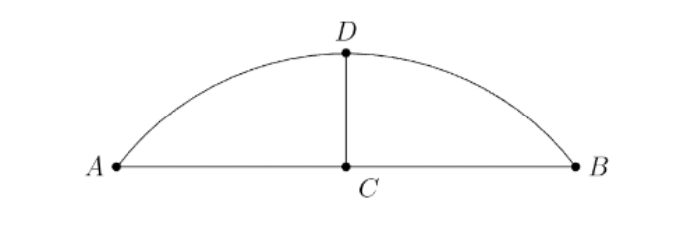
\includegraphics[width=\columnwidth]{olympiad/figs/permo.jpg}
			\caption{}
			\label{fig:plate}
    \end{figure}



    $ C $ is the midpoint of $ AB $, and $ D $ is the midpoint of arc $ AB $. Given that $ AB = 24 $ cm and $ CD = 6 $ cm, what is the radius of the plate in centimeters? (The figure is not drawn to scale.)\hfill(PRMO 2015)
\end{enumerate}
